%************************************************
\chapter{Introduction}\label{ch:introduction}
%************************************************

In recent years, we have witnessed an unprecedented level of presence of technology in our lives. Mobile phones are smarter every day, with computational power that overtakes desktop computers just a couple of years old. At the same time, these devices gain in ubiquity as they extend their functionality to wearable technology, e.g. wearable cameras, wireless earphones or smart watches. The cameras installed in these devices have seen a similar increase in presence, resolution and quality of the lenses and sensors.

The combination of better cameras with improved processing and network connectivity opens the possibilities for computer vision to contribute to diverse applications, some of them having a special role in the inclusivity of people with disabilities and a positive impact in quality of life.

The diagram shown in Figure~\ref{fig:cv_dev_pipeline} illustrates a flow chart that depicts the process behind the development of an application that might depend on computer vision algorithms. In brief, this entails the development of a prototype that is later refined with the use of data. 

Data is the cornerstone for parameter optimisation and at the same time for applying the learning methods that are increasingly being made in many approaches that rely on artificial intelligence. Within computer vision, data, and in particular annotated data, has driven research very strongly. The availability of annotated datasets has achieved prominence, with the organisation of systematic and objective challenges around object recognition and detection; examples include PASCAL VOC \cite{everingham2010pascal} and ImageNet \citep{Deng2009}). Through these data collections and open competitions, benchmarks for performance have been established that are now being extended to other fields within computer vision such as localisation (NAVVIS \cite{Huitl2012} and SLAMbench \cite{nardi2014introducing}.

In recent years, \textit{big data}, or the use of massive amounts of structured and unstructured data has made learning and prediction algorithms an important piece of the artificial intelligence puzzle. However, relying almost entirely in the use of data to solve the problem has sometimes caused the loss of perspective and very poor improvements on performance or none at all \cite{zhu2012we}. It is therefore key to keep developing core algorithms and richer models that help solve artificial intelligence problems by gaining a better understanding of their constraints and representational structure. Often the solution is closer than what we think, and biology can provide us with efficient models that solve the problem in an effective way. In particular, in computer vision, models of the visual system have been shown to be effective in key tasks such as object recognition and visual localisation \cite{lowe2004distinctive,milford2004ratslam}. 


\begin{figure}
\centering
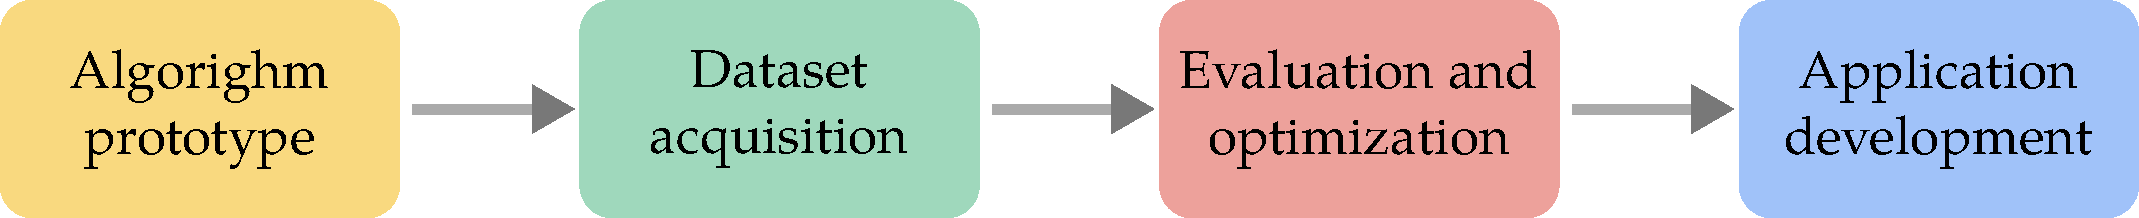
\includegraphics[width=\linewidth]{gfx/Chapter01/cv_dev_pipeline.pdf}
\caption{Stages in the development of a computer vision application. The development of an application in computer vision and similar artificial intelligence disciplines requires a different form of testing compared to the ones seen in standard software engineering toolchains. The use of databases and evaluation and optimisation stages prior to the development of the application complements the typical deterministic behaviour test suites.}
\label{fig:cv_dev_pipeline}
\end{figure}

\section{Mobile visual assistive apps}

Low vision brings many challenges to an individual, including reduced independence and social exclusion. The World Health Organization (WHO) estimates (2012) that more than 285 million people worldwide suffer from low vision or blindness. Due to changing demographics and greater incidence of disease -- e.g. diabetes -- blindness and failing sight are increasing in prevalence.  The cost to society includes direct health care expenditure, care-giver time and lost productivity.  Enabling people with visual impairment to increase participation will help address social exclusion and improve self-esteem and psychological well-being. There is the potential of near-commodity smartphones, backed by appropriate computer vision algorithms and supporting processes, to address this need.

The growth in availability of camera-equipped smartphones, networks, methods of social networking and crowdsourcing of data offers new solutions to develop assistive systems that could be scaled in performance and capability~\cite{Manduchi2012,Worsfold2010}. The services/capabilities that could be offered include:

\emph{Navigation}: Regardless of whether one is outdoors or indoors, navigation in sighted humans relies heavily on the sense of vision~\citep{kalia2008learning,tsuji2005landmarks}. When vision is deteriorated or deprived, a person's ability to navigate -- particularly in unfamiliar settings -- is greatly diminished. Indeed, a significant proportion of individuals who experience sight loss late in life find navigation in unfamiliar environments challenging. This might be a key reason contributing to the fact that more than half (55\%) of the blind and partially sighted in the UK rarely venture outside of their homes \citep{Worsfold2010}. Additionally, GPS does not offer sufficient precision or reliability for indoor manoeuvring. A combination of visual cues, translated into speech or tactile information, is desirable.

\emph{Shopping}: Other challenges include shopping and product recognition, both in shops and at home. The technology for visual object recognition from mobile devices has arrived for sighted users: the challenges to deployment for visually-impaired users includes a) the existence of accessible label databases that are free from commercial bias; b) changing retrieval algorithms and systems to place more emphasis on strong match confidence; c) techniques for conveying information readily to blind and partially-sighted users.

\emph{Personal Safety}: As a partially sighted user, one is faced with a number of hurdles when undertaking journeys away from a familiar environment, and lack of confidence about the ``unseen'' can be a significant contributing factor to reduced mobility.  Where does the pavement end?  Where is the entrance to the bus, and are there stairs?  Are there obstructions at head-height?   

In summary, the overarching need is to increase the possibility for independent living; in a hugely visually-oriented built environment, sighted users rely on visual cues, signage, and recognition of structures such as doorways.  Can these cues be reliably translated into semantically appropriate information using computer vision? Therefore we focus on the feasibility of answering two questions with existing technology from visual cues: ``Where am I?'' and ``What am I holding?''. 
%% 


\section{Appearance-based methods}

In computer vision, image representation methods can be divided in three approaches. Model-based approaches attempt to represent images as a combination of different geometrical shapes, i.e. boxes and circles~\cite{biederman1987}. In contour-based approaches image representations are defined by the edges of the structures present in them~\cite{canny1986computational}. The last approach and subject of this thesis aims to represent visual information by its \textit{appearance}. 

The appearance of an object or a scene in an image can be represented by a series of views from different distances and angles, although usually humans only need a few to recognise more than 30,000 different objects~\cite{biederman1987recognition} solely by their appearance, even when this is partially occluded. 

The set of image representations generated by appearance-based methods are commonly referred as image \textit{features} or \textit{descriptors} since they \textit{describe} properties of the image. Features can be sub-divided into two groups depending on whether they focus on a point or a small area within the images (local approaches) or whether they represent each image in its entirety (global approaches), taking into account all pixels in the image. Good feature traits are robustness against noise, rotation and scale or illumination changes. 

In this thesis, the interest is on local region features. The process to compute these region features is comprised of two steps. In the first one, features that represent one point in the image due to some particular properties of those points are calculated. These are called \textit{interesting points} or \textit{keypoints}. Although keypoints represent interesting points in the image, they can also convey information about the scale and orientation to characterise properties of their
surrounding local region such as stability. Some of the most widely used keypoint detectors are the Harris corner detector~\cite{harris1988combined}, difference of Gaussian (DoG) detector or scale-invariant feature transform (SIFT) keypoint detector~\cite{lowe2004}; and maximally stable extremal regions (MSER) detector~\cite{matas2004robust}.

Once the keypoints have been detected for an image, the next step in order to compute the region features is to perform some image processing algorithms on a patch surrounding the keypoint. The output of this computation is normally stored in a vector, the feature vector or \textit{feature descriptor}. The descriptors include a considerable amount of information about the region and in this thesis we will show that the algorithms to compute them 	are suitable for different tasks.

There is an increasing number of feature description algorithms, with most of the research focusing on the invariability of the descriptors with image transformations (rotation, scale, deformations among others). However, two of them are particularly well known, speeded up robust features (SURF) and especially SIFT, nowadays widely and increasingly extended since its main drawback, the computational load (due to the high dimensionality of its descriptor) is being overcome by the recent advances in multi-core CPUs and particularly graphic processing units (GPU) \cite{Wu2007}. Therefore, it has been used as a baseline method for performance evaluation throughout this thesis.

The image representations achieved by appearance-based approaches can be used for a multitude of artificial intelligence tasks: object recognition, visual localisation, scene detection, face recognition, human identification and action recognition to name only a few. As mentioned in the previous section, this thesis will cover the first two applications, object recognition and visual localisation, with emphasis in the challenging scenarios of hand-held image acquisition and assistive applications. My hypothesis in this aspect is that appearance-based methods can be, in isolation, valid solutions for many challenging problems simultaneously, and combined with other sensing (e.g. WiFi, inertial and depth sensors) and inference techniques (e.g. tracking) it can be a complementary technology that help improve the overall performance of the different approaches on their own. Specifically, as a means to test this hypothesis, it is also my goal to evaluate which appearance-based techniques adapt better to the needs of hand-held object recognition and visual navigation in terms of accuracy, power, time and computational load and assess their room for performance.

\section{Biological evidence of place cell visual localisation} 

Place cell behaviour is usually found by obtaining electrical recordings from several biological neurons (CA1) in specific regions of the hippocampus; by comparing firing rates between neurons and relative to background firing rates, one can infer which neurons are displaying place-cell behaviour. The concept of a biological place cell (BPC) is illustrated in Figure~\ref{fig:Maze}.  The coloured circles depict locations within a maze in which individual place cells show elevated firing relative to other place cells.  Through observing this electrical behaviour over many trials, firing patterns can be decoded, and used as an indication of where the rat is along the maze: in the simplest case, the BPC which fires maximally is taken as the rat's approximate location in space. 

\begin{figure}[!t]
\centering
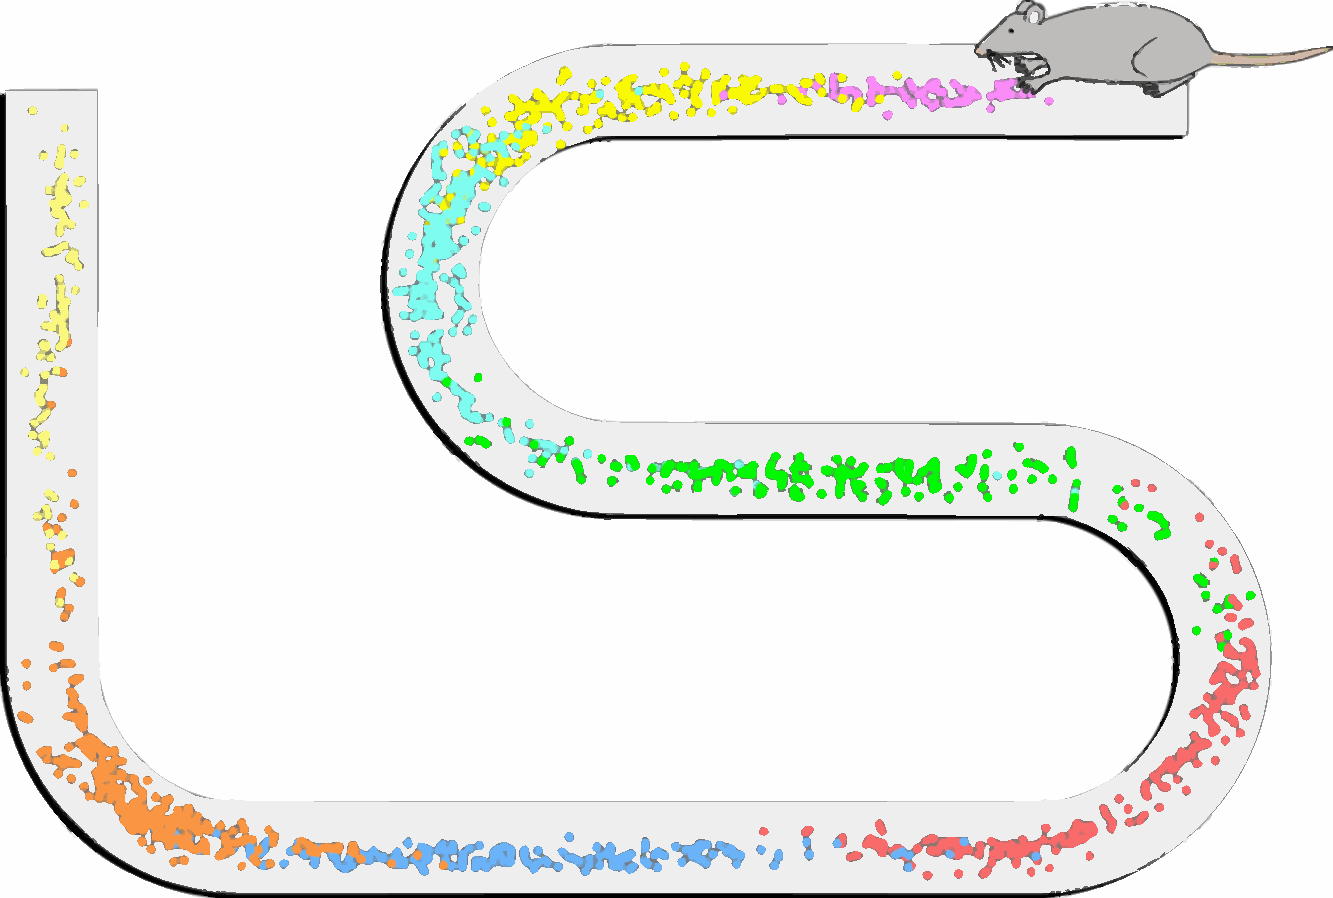
\includegraphics[width=.6\linewidth]{./gfx/Chapter01/bio_place_cells_rat.pdf}
\caption{Illustration of place cells; this figure is from experiments of S.P. Layton in behaving rats. Small coloured circles depict individual biological place-cells having maximum activation (firing rate) compared to all other place cells throughout the navigation space. Licensed for use under the Creative Commons Attribution-ShareAlike 3.0 License.}
\label{fig:Maze}
\end{figure}

There is no suggestion that the inference in place cells is purely a binary form of ``you are here'' type of response.  Instead, it is likely that the firing rates of several place cells are combined to more accurately infer position \cite{hafting2005microstructure}, a process that might involve both phase-locked patterns of firing and rate codes \cite{dragoi2006temporal}. Place cell selectivity itself is thought to arise from a combination of inputs and cell responses inside and outside hippocampal areas. Rate coding \cite{van2001rate} is just one mechanism by which groups of neurons are thought to encode and represent sensory information. A rate code can be interpreted by estimating average firing rates (over trials) within the same neuron. 
The visual information captured by the eyes of an animal should be seen as only one of the many sensory and internal cues that lead to the spatially selective nature of biological place-cell responses \cite{hassabis2009decoding}. Nevertheless, in many animals, and certainly in humans and primates, vision is a particularly strong cue as to one's position \cite{epstein1998cortical}, therefore another research hypothesis for this thesis is whether place cells can be modelled with appearance-based methods and be used for inferring locations by only using visual input.


\section{Objectives}

The main goal of this work is to investigate, formulate, implement and evaluate appearance-based methods that might provide a better representation of the visual inputs produced in the contexts of hand-held object recognition and visual localisation. To this end, six principal objectives have been set


\begin{enumerate}
%% ch02

\item \textbf{Chapter 2} In this chapter I present the preliminary work carried out to evaluate the requirements of computer vision Apps in the challenging contexts of hand-held and wearable object recognition and visual localisation, with emphasis in the assistive use case for the blind and partially sighted. These two applications are intended to help provide answers to the questions of ``Where am I?'' and ``What am I holding?''.

I provide pilot studies of appearance-based methods for these applications and analyse the research hypothesis and requirements to fulfil them. These studies motivated the work described in subsequent chapters and represent the first prototypes of the methods proposed in this thesis and large benchmarking datasets that were acquired to provide performance evaluations.

In particular, this pilot work provides two main contributions: it suggests that it is possible to estimate indoor localisation of a user solely by using the input acquired with a smartphone or wearable camera. Here I also define the concept of ``visual path'', or user-crowdsourced videos of indoor journeys and their descriptions of visual appearance. Finally, I describe the first analysis and prototype data acquisition for hand-held object recognition using appearance-based methods.

%% ch03

\item \textbf{Chapter 3} The hypothesis for the work described in this chapter originates from visual object recognition as an application of camera-equipped smartphones. The ability to recognise objects through photos taken with wearable and handheld cameras is already possible through some of the larger internet search providers; yet, there is little rigorous analysis of the quality of search results, particularly where there is great disparity in image quality. This chapter describes the development of the Small Hand-held Object Recognition Test (SHORT). This includes a dataset that is suitable for recognising hand-held objects from either snapshots or videos acquired using hand-held or wearable cameras. SHORT provides a collection of images and ground truth that help evaluate the different factors that affect recognition performance. At its present state, the dataset is comprised of a set of high quality training images and a large set of nearly 135,000 smartphone-captured test images of 30 grocery products. In this chapter I also discuss some open challenges in the visual object recognition of objects that are being held by users. I evaluate the performance of a number of popular object recognition algorithms, with differing levels of complexity, when tested against SHORT.

%% ch04

\item \textbf{Chapter 4} In this chapter I address a specific use-case of wearable or hand-held camera technology related to indoor navigation. The main research question is whether it is possible to crowdsource navigational data in the form of video sequences captured from wearable cameras.  This work uses the foundation provided in Chapter~\ref{ch:chapter2} to test video data for navigational content, and algorithms for extracting that content without using geometric inference techniques (such as simultaneous localisation and mapping, (SLAM)).  Tracking is not included in this evaluation as the purpose is to explore the hypothesis that visual content, on its own, contains cues that can be mined to infer a person's location.  This hypothesis is tested through estimating the positional error inferred during one journey with respect to other journeys along the same approximate path.

The contributions described in this chapter are threefold. First, I propose alternative methods for video feature extraction that identifies candidate matches between query sequences against a database of previously acquired sequences. Secondly, I describe an evaluation methodology that estimates the error distributions in position inference with respect to the ground truth. In the evaluation standard approaches are compared in the retrieval context, such as SIFT and HOG3D, to establish positional estimates. The final contribution is a publicly available database (the RSM dataset) comprising over 150,000 frames of video sequences with positional ground-truth in the form of position along a path. The data was acquired along more than 3 km worth of indoor journeys with a hand-held device (Nexus 4) and a wearable device (Google Glass).

Finally, I describe experimental results showing that image queries against previously acquired visual paths could contribute to positional estimates used in navigation. The error performance using only these appearance-based methods is favourable when compared with a state-of-the-art SLAM method, LSD-SLAM, even without the use of a motion model. The evaluation also yields that single-frame query methods work better than spatio-temporal queries in the context of these tests which do not use explicit tracking or self-motion estimation. 

%% ch05
\item \textbf{Chapter 5} In the work described in this chapter I used visual information from wearable and hand-held cameras in order to reproduce the rate-coding effect found in mammalian place cells. These models receive the name of artificial place cells (APCs). 

I also evaluated the accuracy of localisation by creating APCs using different visual descriptors and place cell widths. The results on visual localisation are reported on the RSM dataset described in Chapter~\ref{ch:chapter4} and compared with LSD-SLAM, showing favourable results. I tested localisation using two methods: the maximum response of a particular APC; and using a joint coding approach that employs a generalised regression neural network (GRNN) to provide sub-cell localisation.

\item \textbf{Chapter 6} This chapter describes an assistive vision-based localisation App that uses a wearable camera and a haptic feedback tablet to provide basic positional information. The \textit{back-end} of this prototype App uses one of the appearance-based methods described in Chapter~\ref{ch:chapter4}, whilst the \textit{front-end} aims to provide feedback using a modified commercial Android tablet able to provide tactile cues to the user. I also describe the experiments carried out with 18 subjects on the quality of tactile feedback to convey localisation to non-sighted users.

\item \textbf{Chapter 7} Finally, this chapter provides my concluding remarks while summarising the main contributions of this dissertation and future work.
